\documentclass[journal]{IEEEtran}

\usepackage{blindtext}
\usepackage{algorithm}
\usepackage{algorithmic}
\usepackage{cite}
\usepackage{graphicx}
\usepackage{array}
\usepackage{color}
\usepackage{tabularx}
\usepackage{epsfig}
\usepackage{amsmath}
\usepackage{amssymb}
\usepackage{bm}
\usepackage{wasysym}
\usepackage{circuitikz}
\usepackage{float}
\usetikzlibrary{arrows,shapes,calc,positioning}

\newcommand{\myscope}[2]
{\draw[thick,rotate=#2] (#1) circle (12pt)
(#1) ++(-0.35,-0.1) --++ (0.3,0.3) --++ (0,-0.3) --++(0.3,0.3) --++(0,-0.3);}

\begin{document}

\title{CSCE 221 \\ Checkpoint 5 Revision}

\author{Jacob~Purcell,~\IEEEmember{Texas~A\&M,~Student}}

\maketitle

\section*{Question 2}

    \subsection*{1.}
    I didn't know what the BST ADT operations were so I guessed,
    After research I found that the operations are $\boxed{MakeEmpty,~Find,~FindMin,~FindMax,~Delete}$.

    \subsection*{2.}
    If the BST is linear, it is a linked list so all operation assume $\boxed{O(N)}$ since they require iterating through every element.

    \subsection*{3.}
    Each requires traversing a tree recursively so they would be $O(N)$.

    \subsection*{4.}
    Since 1 is the smallest value and the tree is produced with a random permutation of elements, 1 would be at the bottom of the left most subtree of the root.
    Keep following the left child and eventually we will get to 1.

    \subsection*{5.}
    Since N is the largest value and the tree is produced with a random permutation of elements, N would be at the bottom of the right most subtree of the root.
    Keep following the right child and eventually we will get to N.


    \subsection*{6.}
    Since 4 is inserted first, $\boxed{4 is the root}$.

    \subsection*{7.}
    Using 
    \begin{equation}
        \frac{n+1}{2}
    \end{equation}
    we have $\boxed{7}$ leaf nodes when n = 13.

    \subsection*{8.}
    Solving for N,
    $$ I + \frac{N+1}{2} = N $$
    $$ 2I + 1 = N,~I=12 $$
    $$\boxed{N=25}$$

\section*{Question 4}
I did incorrect pointer reassignments. The correct deletions go as follows,
\begin{figure}[H]
    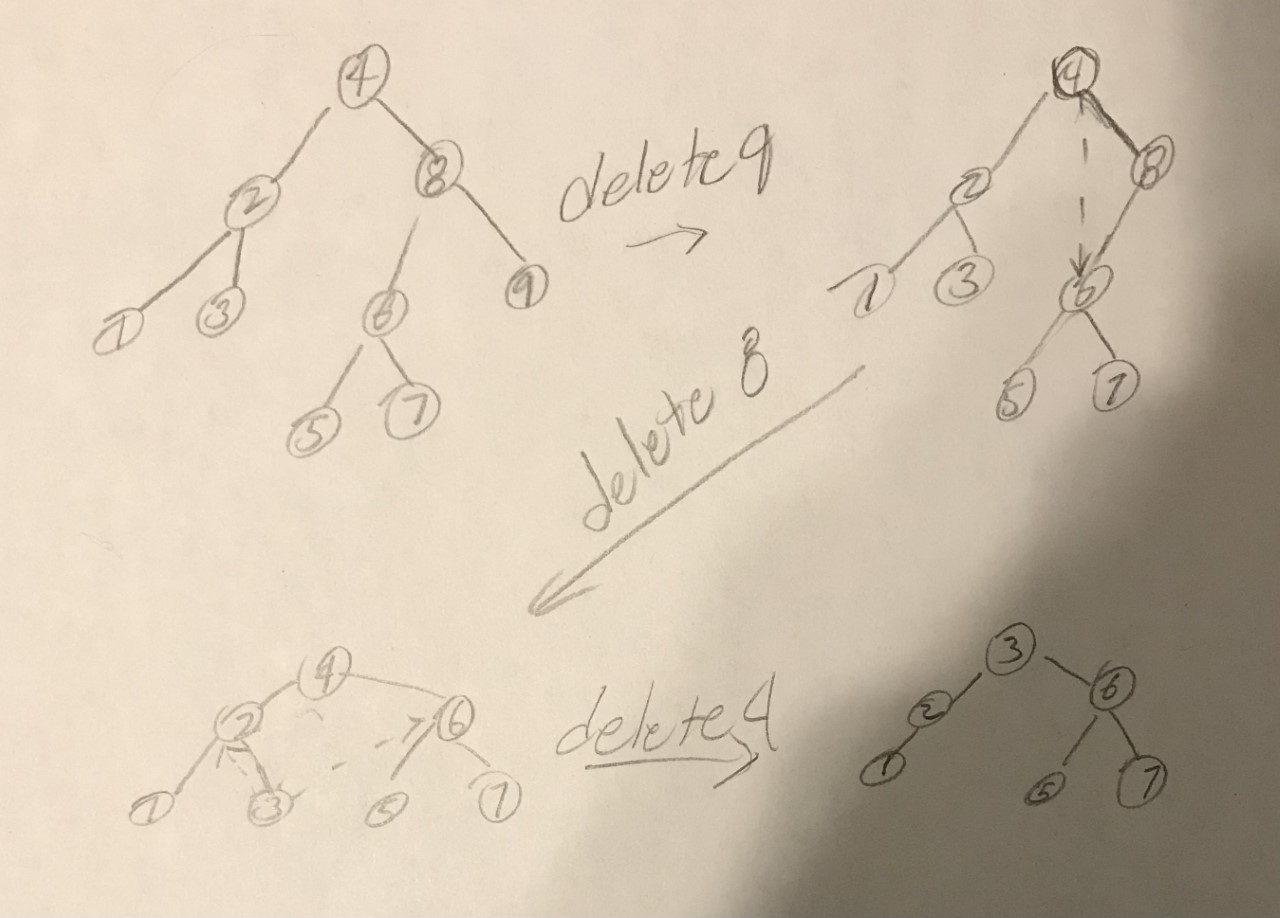
\includegraphics[scale = 0.17]{tree.png}
    \caption{Deletion sequence for given tree.}
\end{figure}

\section*{Question 5}
I guessed the meaning of each tree traversal, after finding out what these traversal orders mean,
the following answers were reached,

\subsection*{1.}
$$Preorder:~RAVXBNE$$

\subsection*{2.}
$$Postorder:~XBVNAER$$

\subsection*{3.}
$$Inorder:~XVBANRE$$

\subsection*{4.}
$$Levelorder:~RAEVNXB$$

\end{document}
